\documentclass[12pt]{beamer}
\usepackage{../latex-sty/mypres}
\usepackage[utf8]{inputenc}
\usepackage[T2A]{fontenc}
\usepackage[russian]{babel}

\expandafter\def\expandafter\insertshorttitle\expandafter{%
  \insertshorttitle\hfill%
  \insertframenumber\,/\,\inserttotalframenumber}
\title[Семинар 9]{Методы оптимизации. \\
 Семинар 9. Условия оптимальности.}
\author{Александр Катруца}
\institute{Московский физико-технический институт\\
Факультет Управления и Прикладной Математики} 
\date{\today}

\begin{document}
\begin{frame}
\maketitle
\end{frame}

\begin{frame}{Напоминание}
\begin{itemize}
\item Сопряжённые функции
\item Неравенство Юнга-Фенхеля
\item Примеры сопряжённых функций
\end{itemize}
\end{frame}

\begin{frame}{Мотивация}

\begin{block}{Вопрос 0}
Когда существует решение оптимизационной задачи?
\end{block}

\begin{block}{Вопрос 1}
Как проверить, что точка является решением оптимизационной задачи? 
\end{block}

\begin{block}{Вопрос 2}
Из каких условий можно найти решение оптимизационной задачи?
\end{block}

\end{frame}

\begin{frame}{Существование решения}
\begin{block}{Теорема Вейерштрасса}
Пусть $X \subset R^n$ компактное множество и пусть $f(x)$ непрерывная функция на $X$. 
Тогда точка глобального минимума функции $f (x)$ на $X$ существует.
\end{block}

Эта теорема гарантирует, что решение подавляющего большинства разумных задач существует.
 
\end{frame}

\begin{frame}{Условия оптимальности}
\begin{block}{Определение}
Условием оптимальности будем называть некоторое выражение, выполнимость которого даёт необходимое и (или) достаточное условие экстремума. 
\end{block}
Классы задач:
\begin{itemize}
\item Общая задача минимизации
\item Задача безусловной минимизации
\item Задача минимизации с ограничениями типа равенств
\item Задача минимизации с ограничениями типа равенств и неравенств
\end{itemize}
\end{frame}

\begin{frame}{Общая задача минимизации}

\begin{block}{Задача}
\[
f(x) \rightarrow \min\limits_{{\color{red}{x \in X}}}
\]
\end{block}

\begin{block}{Критерий оптимальности}
Пусть $f(x)$ определена на множестве $X \subset \bbR^n$.
Тогда 
\begin{enumerate}
\item если $x^*$ точка минимума $f(x)$ на $X$, то $0 \in \partial_X f(x^*)$
\item если для некоторой точки $x^* \in X$ существует субдифференциал $\partial_X f(x^*)$ и $0 \in \partial_X f(x^*)$, то $x^*$~--- точка минимума $f(x)$ на $X$.
\end{enumerate}
\end{block}
Какие недостатки у приведённого критерия?

\end{frame}

\begin{frame}{Примеры}
\begin{itemize}
\item $\bx^{\T}\bx + \alpha \| \bx - 
\bc \|_2 \rightarrow \min\limits_{\bx \in \bbR^n}$, $\alpha > 0$
\item $\bx^{\T}\bx + \alpha \| \bc^{\T}\bx - 
b \|_2 \rightarrow \min\limits_{\bx \in \bbR^n}$, $\alpha > 0$
\item Ограничение на допустимое множество
\begin{equation*}
\begin{split}
\vspace{-4mm}
&(x + 2)^2 + |y + 3| \rightarrow \min\limits_{(x, y) \in \bbR^2}\\
\text{s.t. }& 8 + 2x - y \leq 0
\end{split}
\end{equation*}
\end{itemize}
\end{frame}

\begin{frame}{Задача безусловной минимизации}
Задача: $f(x) \rightarrow \min\limits_{\color{red}{x \in \bbR^n}}$.

\begin{block}{Критерий оптимальности для выпуклых функций}
Пусть $f(x)$ выпуклая функция на $\bbR^n$. 
Тогда точка $x^*$ решение задачи безусловной минимизации $\Leftrightarrow$ $0 \in \partial f(x^*)$.
\end{block}

\begin{block}{Следствие}
Если $f(x)$ выпукла и дифференцируема на $\bbR^n$.
Тогда точка $x^*$ решение задачи безусловной минимизации $\Leftrightarrow$ $\nabla f(x^*) = 0$.
\end{block}

\begin{block}{Достаточное условие для невыпуклых функций}
Пусть $f$ дважды дифференцируема на $\bbR^n$ и $x^*$ такая что $\nabla f(x^*) = 0$. 
Тогда если $\nabla^2 f(x^*) \succ 0$, то $x^*$ точка строгого локального минимума $f(x)$ на $\bbR^n$.  
\end{block}

\end{frame}

\begin{frame}{Примеры}
\begin{itemize}
\item $x_1e^{x_1} - (1 + e^{x_1})\cos x_2 \rightarrow \min$
\item Функция Розенброка: $(1 - x_1)^2 + \alpha \sum\limits_{i = 2}^n (x_i - x^2_{i-1})^2 \rightarrow \min$, $\alpha > 0$
\item $x^2_1 + x^2_2 - x_1x_2 + e^{x_1 + x_2} \rightarrow \min$
\end{itemize}
\end{frame}

\begin{frame}{{\small Задача минимизации с ограничениями типа равенств}}

\begin{block}{Задача}
\vspace{-3mm}
\begin{equation*}
\begin{split}
& f(x) \rightarrow \min\limits_{x \in \bbR^n} \\
\text{s.t. } & g_i(x) = 0, \; i = 1,\ldots, m 
\end{split}
\end{equation*}
\end{block}

\begin{block}{Лагранжиан}
\vspace{-2mm}
\begin{equation*}
L(x, \blambda) = f(x) + \sum\limits_{i=1}^m\lambda_i g_i(x)
\end{equation*}
\end{block}

%\begin{block}{Критерий оптимальности}
%Пусть $f(x)$ и $g_i(x)$ дважды дифференцируемы в точке $x^*$ и непрерывно дифференцируемы в некоторой окрестности $x^*$.
%Пусть также $\nabla_x L(x^*, \blambda) = 0$.
%Тогда если $\bh^{\T}\nabla^2 L(x^*, \blambda)\bh > 0$, где $\bh \in T(\bx^*|G)$~--- касательный конус, то $x^*$~--- точка локального минимума.
%\end{block}

\end{frame}

\begin{frame}{Возможные варианты}
\begin{figure}
\centering
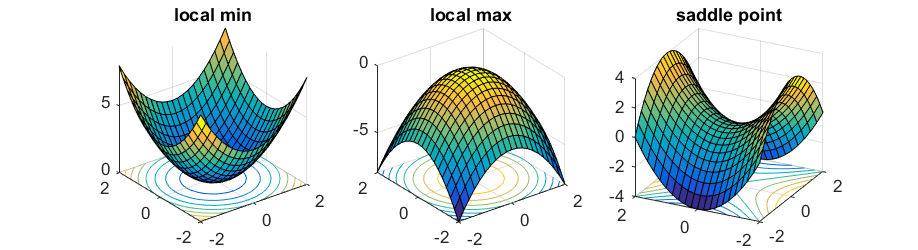
\includegraphics[scale=0.5]{minmaxsaddle.png}
\caption{Рисунок взят из блога \url{http://www.offconvex.org/2016/03/22/saddlepoints/}}
\end{figure}
\end{frame}

\begin{frame}{Примеры}
\begin{itemize}
\item $\sum\limits_{i=1}^n\alpha_i x^4_i \rightarrow \extr\limits_{\bx \in G}$, $G = \{\bx \in \bbR^n \; | \; \bc^{\T}\bx = 1 \}$, $\alpha_i > 0,\; c_i > 0$
%\item $x_1 + 4x_2 + 9x_3 \rightarrow \extr\limits_{\bx \in G}, \; G = \left \{ \frac{1}{x_1} + \frac{1}{x_2} + \frac{1}{x_3} = 1 \right\}$
\end{itemize}
\end{frame}

\begin{frame}{{\small Задача минимизации с ограничениями типа равенств и неравенств}}

\begin{block}{Задача}
\vspace{-5mm}
\begin{equation*}
\begin{split}
& \min\limits_{x \in \bbR^n} f(x)\\
\text{s.t. } & g_i(x) = 0, \; i = 1,\ldots,m\\
& h_j(x) \leq 0, \; j = 1,\ldots, p
\end{split}
\end{equation*}
\end{block}

\begin{block}{Лагранжиан}
\begin{equation*}
L(x, \blambda, \bmu) = f(x) + \sum\limits_{i=1}^m\lambda_i g_i(x) + \sum\limits_{j=1}^p \mu_j h_j(x)
\end{equation*}
\end{block}
\end{frame}

\begin{frame}{Условия оптимальности Каруша-Куна-Таккера (ККТ)}
\begin{block}{Необходимые условия}
Пусть для задачи выполнено условие регулярности. Тогда если $x^*$ локальное решение задачи, и функции $f, h_j, g_i$ дифференцируемы, то найдутся такие $\bmu^*$ и $\blambda^*$, для которых выполнено следующее:
\begin{itemize}
\item $g_i(x^*) = 0$, $i = 1,\ldots,m$
\item $h_j(x^*) \leq 0$, $j = 1,\ldots,p$
\item $ \mu^*_j \geq 0$, $j = 1,\ldots,p$
\item $\mu^*_jh_j(x^*) = 0$, $j = 1,\ldots,p$
\item $\nabla_x L(x^*, \blambda^*, \bmu^*) = 0$
\end{itemize}
\end{block}
Если задача выпуклая, то эти же условие является достаточным.
\end{frame}

\begin{frame}{Примеры условий регулярности}
\begin{itemize}
\item Если $g_i$ и $h_j$ линейны, то дополнительные условия не нужны
\item Градиенты ограничений типа равенств и активных ограничений типа неравенств линейно независимы в~$x^*$
\item Условие Слейтера:
\begin{itemize}
\item Задача является выпуклой, то есть $g_i$~--- аффинные, $h_j$ и $f$~--- выпуклые
\item Существует точка $x_0$ такая что $g_i(x_0) = 0$ и $h_j(x_0) < 0$
\end{itemize}

\end{itemize}
\end{frame}

%\begin{frame}{Условия оптимальности (cont'd)}
%\small
%Если задача невыпуклая, то
%\begin{block}{Достаточное условие первого порядка}
%\small
%Если для стационарной точки $(x^*, \blambda^*, \bmu^*)$ число активных неравенств $|J|$ такое что $n = m + |J|$ и $\mu_j > 0, \; j \in J$, то эта точка является точкой минимума.
%\end{block}
%
%\begin{block}{Достаточное условие второго порядка}
%\small
%Если в задаче математического программирования число активных ограничений меньше размерности задачи, то точка $x^*$ является решением задачи, если выполнены условия
%\vspace{-3mm}
%\[
%\bz^{\T}\nabla_{xx}^2 L(x^*)\bz > 0
%\vspace{-3mm}
%\] 
%для 
%\vspace{-4mm}
%\begin{itemize}
%\item $\bz \neq 0$ и $\nabla g^{\T}_i(x^*)\bz = 0$
%\vspace{-3mm}
%\item при $j \in J$ и $\mu_j > 0$, $\nabla h^{\T}_j(x^*) \bz = 0$
%\vspace{-3mm}
%\item при $j \in J$ и $\mu_j = 0$, $\nabla h^{\T}_j(x^*) \bz \leq 0$
%\end{itemize}
%\end{block}
%
%\end{frame}

\begin{frame}{Примеры}
\begin{itemize}
\item 
\begin{equation*}
\begin{split}
& \min x + 3y\\
\text{s.t. } & x - y \geq 0\\
& (x - 1)^2 + (y - 1)^2 \leq 9
\end{split}
\end{equation*}
\item 
\begin{equation*}
\begin{split}
& \min \; (x+ 1)^2 + (y + 1)^2\\
\text{s.t. } & 2x + 3y \geq 5
\end{split}
\end{equation*}
\item 
\begin{equation*}
\begin{split}
& \min \; x_1 - 2x_2 + x_3\\
\text{s.t. } & -x_1 + x_2 + x_3 \leq -2\\
& x_1 + 2x_2 + x_3 \leq 10\\
& x_1 + x_2 - x_3 = 4\\
& x_i \geq 0
\end{split}
\end{equation*}
%\small
%\item Пример 1
%\vspace{-5mm}
%\begin{equation*}
%\begin{split}
%& \extr (x_1 - 3)(x_2 - 2)\\
%\text{s.t. } & x_1 + 2x_2 = 4\\
%& x^2_1 + x^2_2 \leq 5\\
%& x_1 \geq 0, \; x_2 \geq 0 
%\end{split}
%\end{equation*} 
%\vspace{-5mm}
%\item Пример 2
%\vspace{-5mm}
%\begin{equation*}
%\begin{split}
%& \extr \sum\limits_{i=1}^n \frac{c_i}{x_i}\\
%\text{s.t. } & \sum\limits_{i=1}^n a_ix_i \leq b\\
%& x_i > 0, \; b > 0, \; c_i > 0, \; a_i > 0
%\end{split}
%\end{equation*}
%\vspace{-4mm}
%\item Пример 3
%\vspace{-3mm}
%\begin{equation*}
%\begin{split}
%& \extr (x_1x_3 - 2x_2)\\
%\text{s.t. } & 2x_1 - x_2 - 3x_3 \leq 10\\
%& 3x_1 + 2x_2 + x_3 = 6\\
%& x_2 \geq 0
%\end{split}
%\end{equation*}
\end{itemize}
\end{frame}

\begin{frame}{Резюме}
\begin{itemize}
\item Существование решения оптимизационной задачи 
\item Условия оптимальности для
\begin{itemize}
\item общей задачи оптимизации
\item задачи безусловной оптимизации
\item задачи оптимизации с ограничениями типа равенств
\item задачи оптимизации с ограничениями типа равенств и неравенств
\end{itemize}
\end{itemize}
\end{frame}
\end{document}
